\documentclass{article}
\usepackage[margin=1in]{geometry}
\usepackage[linesnumbered,ruled,vlined]{algorithm2e}
\usepackage{amsfonts}
\usepackage{amsmath}
\usepackage{amssymb}
\usepackage{amsthm}
\usepackage{enumitem}
\usepackage{fancyhdr}
\usepackage{hyperref}
\usepackage{minted}
\usepackage{multicol}
\usepackage{pdfpages}
\usepackage{standalone}
\usepackage[many]{tcolorbox}
\usepackage{tikz-cd}
\usepackage{transparent}
\usepackage{xcolor}
% \tcbuselibrary{minted}

\author{Nathan Solomon}

\newcommand{\fig}[1]{
    \begin{center}
        \includegraphics[width=\textwidth]{#1}
    \end{center}
}

% Math commands
\renewcommand{\d}{\mathrm{d}}
\DeclareMathOperator{\id}{id}
\DeclareMathOperator{\im}{im}
\DeclareMathOperator{\proj}{proj}
\DeclareMathOperator{\Span}{span}
\DeclareMathOperator{\Tr}{Tr}
\DeclareMathOperator{\tr}{tr}
\DeclareMathOperator{\ad}{ad}
\DeclareMathOperator{\ord}{ord}
%%%%%%%%%%%%%%% \DeclareMathOperator{\sgn}{sgn}
\DeclareMathOperator{\Aut}{Aut}
\DeclareMathOperator{\Inn}{Inn}
\DeclareMathOperator{\Out}{Out}
\DeclareMathOperator{\stab}{stab}

\newcommand{\N}{\ensuremath{\mathbb{N}}}
\newcommand{\Z}{\ensuremath{\mathbb{Z}}}
\newcommand{\Q}{\ensuremath{\mathbb{Q}}}
\newcommand{\R}{\ensuremath{\mathbb{R}}}
\newcommand{\C}{\ensuremath{\mathbb{C}}}
\renewcommand{\H}{\ensuremath{\mathbb{H}}}
\newcommand{\F}{\ensuremath{\mathbb{F}}}

\newcommand{\E}{\ensuremath{\mathbb{E}}}
\renewcommand{\P}{\ensuremath{\mathbb{P}}}

\newcommand{\es}{\ensuremath{\varnothing}}
\newcommand{\inv}{\ensuremath{^{-1}}}
\newcommand{\eps}{\ensuremath{\varepsilon}}
\newcommand{\del}{\ensuremath{\partial}}
\renewcommand{\a}{\ensuremath{\alpha}}

\newcommand{\abs}[1]{\ensuremath{\left\lvert #1 \right\rvert}}
\newcommand{\norm}[1]{\ensuremath{\left\lVert #1\right\rVert}}
\newcommand{\mean}[1]{\ensuremath{\left\langle #1 \right\rangle}}
\newcommand{\floor}[1]{\ensuremath{\left\lfloor #1 \right\rfloor}}
\newcommand{\ceil}[1]{\ensuremath{\left\lceil #1 \right\rceil}}
\newcommand{\bra}[1]{\ensuremath{\left\langle #1 \right\rvert}}
\newcommand{\ket}[1]{\ensuremath{\left\lvert #1 \right\rangle}}
\newcommand{\braket}[2]{\ensuremath{\left.\left\langle #1\right\vert #2 \right\rangle}}

\newcommand{\catname}[1]{{\normalfont\textbf{#1}}}

\newcommand{\up}{\ensuremath{\uparrow}}
\newcommand{\down}{\ensuremath{\downarrow}}

% Custom environments
\newtheorem{thm}{Theorem}[section]

\definecolor{probBackgroundColor}{RGB}{250,240,240}
\definecolor{probAccentColor}{RGB}{140,40,0}
\newenvironment{prob}{
    \stepcounter{thm}
    \begin{tcolorbox}[
        boxrule=1pt,
        sharp corners,
        colback=probBackgroundColor,
        colframe=probAccentColor,
        borderline west={4pt}{0pt}{probAccentColor},
        breakable
    ]
    \color{probAccentColor}\textbf{Problem \thethm.} \color{black}
} {
    \end{tcolorbox}
}

\definecolor{exampleBackgroundColor}{RGB}{212,232,246}
\newenvironment{example}{
    \stepcounter{thm}
    \begin{tcolorbox}[
      boxrule=1pt,
      sharp corners,
      colback=exampleBackgroundColor,
      breakable
    ]
    \textbf{Example \thethm.}
} {
    \end{tcolorbox}
}

\definecolor{propBackgroundColor}{RGB}{255,245,220}
\definecolor{propAccentColor}{RGB}{150,100,0}
\newenvironment{prop}{
    \stepcounter{thm}
    \begin{tcolorbox}[
        boxrule=1pt,
        sharp corners,
        colback=propBackgroundColor,
        colframe=propAccentColor,
        breakable
    ]
    \color{propAccentColor}\textbf{Proposition \thethm. }\color{black}
} {
    \end{tcolorbox}
}

\definecolor{thmBackgroundColor}{RGB}{235,225,245}
\definecolor{thmAccentColor}{RGB}{50,0,100}
\renewenvironment{thm}{
    \stepcounter{thm}
    \begin{tcolorbox}[
        boxrule=1pt,
        sharp corners,
        colback=thmBackgroundColor,
        colframe=thmAccentColor,
        breakable
    ]
    \color{thmAccentColor}\textbf{Theorem \thethm. }\color{black}
} {
    \end{tcolorbox}
}

\definecolor{corBackgroundColor}{RGB}{240,250,250}
\definecolor{corAccentColor}{RGB}{50,100,100}
\newenvironment{cor}{
    \stepcounter{thm}
    \begin{tcolorbox}[
        enhanced,
        boxrule=0pt,
        frame hidden,
        sharp corners,
        colback=corBackgroundColor,
        borderline west={4pt}{0pt}{corAccentColor},
        breakable
    ]
    \color{corAccentColor}\textbf{Corollary \thethm. }\color{black}
} {
    \end{tcolorbox}
}

\definecolor{lemBackgroundColor}{RGB}{255,245,235}
\definecolor{lemAccentColor}{RGB}{250,125,0}
\newenvironment{lem}{
    \stepcounter{thm}
    \begin{tcolorbox}[
        enhanced,
        boxrule=0pt,
        frame hidden,
        sharp corners,
        colback=lemBackgroundColor,
        borderline west={4pt}{0pt}{lemAccentColor},
        breakable
    ]
    \color{lemAccentColor}\textbf{Lemma \thethm. }\color{black}
} {
    \end{tcolorbox}
}

\definecolor{proofBackgroundColor}{RGB}{255,255,255}
\definecolor{proofAccentColor}{RGB}{80,80,80}
\renewenvironment{proof}{
    \begin{tcolorbox}[
        enhanced,
        boxrule=1pt,
        sharp corners,
        colback=proofBackgroundColor,
        colframe=proofAccentColor,
        borderline west={4pt}{0pt}{proofAccentColor},
        breakable
    ]
    \color{proofAccentColor}\emph{\textbf{Proof. }}\color{black}
} {
    \qed \end{tcolorbox}
}

\definecolor{noteBackgroundColor}{RGB}{240,250,240}
\definecolor{noteAccentColor}{RGB}{30,130,30}
\newenvironment{note}{
    \begin{tcolorbox}[
        enhanced,
        boxrule=0pt,
        frame hidden,
        sharp corners,
        colback=noteBackgroundColor,
        borderline west={4pt}{0pt}{noteAccentColor},
        breakable
    ]
    \color{noteAccentColor}\textbf{Note. }\color{black}
} {
    \end{tcolorbox}
}


\fancyhf{}
\setlength{\headheight}{24pt}

\date{\today}
\title{Physics 127 Homework \#5}

\begin{document}
\maketitle

\begin{prob}
\end{prob}
The Faraday tensor is defined as
\[ F_{\mu \nu} := \partial_\mu A_\nu - \partial_\nu A_\mu. \]
So after the gauge transformation $A_\mu \rightarrow A_\mu + \partial_\mu \lambda$, that becomes
\[ F_{\mu \nu} := \partial_\mu (A_\nu + \partial_\nu \lambda) - \partial_\nu (A_\mu + \partial_\mu \lambda), \]
which simplifies to
\[ F_{\mu \nu} = \partial_\mu A_\nu + \partial_\mu \partial_\nu \lambda - \partial_\nu A_\mu - \partial_\nu \partial_\mu \lambda = F_{\mu \nu} + (\partial_\mu \partial_\nu - \partial_\nu \partial_\mu) \lambda = F_{\mu \nu}, \]
so $F_{\mu \nu}$ is invariant.
\par
Suppose we want to choose $\lambda(x)$ such that $A'_\mu = A_\mu + \partial_\mu \lambda$ satisfies $\partial_\mu A'^\mu = 0$. Then
\[ \partial_\mu (A^\mu + \partial^\mu \lambda) = 0. \]
Such a $\lambda(x)$ can always be constructed, so there is always a gauge in which $\partial_\mu A^\mu = 0$. In that gauge, the equation $\partial_\mu F^{\mu \nu} = 0$ becomes
\begin{align*}
    0 &= \partial_\mu (\partial^\mu A^\nu - \partial^\nu A^\mu) \\
      &= \partial_\mu \partial^\mu A^\nu - \partial^\nu \partial_\mu A^\mu \\
      &= \Box A^\nu - \partial^\nu 0 \\
      &= \Box A^\mu.
\end{align*}

\bigskip
\par
\begin{prob}
\end{prob}
The Lagrangian density is
\begin{align*}
    \mathcal{L} &= - \frac{1}{4} F^{\mu \nu} F_{\mu \nu} \\
                &= - \frac{1}{4} \left( F^{00}F_{00} + F^{i0}F_{i0} + F^{0j}F_{0j} + F^{ij}F_{ij} \right) \\
                &= - \frac{1}{4} \left( 0 \cdot 0 + F^{i0}F_{i0} + F^{0j}F_{0j} + F^{ij}F_{ij} \right)  \\
                &= - \frac{1}{4} \left( (E^i) (E_i) + (-E^j)(-E_j) + (-\varepsilon^{ijk}B_k) (-\varepsilon_{ijk}B^k) \right)  \\
                &= - \frac{1}{4} \left( -2 E \cdot E + (\varepsilon^{ijk} \varepsilon_{ijk})(B_k B^k) \right)  \\
                &= - \frac{1}{4} \left( -2 E^2 + 2 B_k B^k \right)  \\
                &= \frac{1}{2} \left( E^2 - B^2 \right).
\end{align*}
If $A^\mu$ changes by a small amount $\delta A^\mu$ (meaning terms containing $\delta^2$ can be ignored), then the action changes by
\begin{align*}
    \delta S &= \left( - \frac{1}{4} \int (\partial^\mu (A^\nu + \delta A^\nu) - \partial^\nu (A^\mu + \delta A^\mu)) (\partial_\mu (A_\nu + \delta A_\nu) - \partial_\nu (A_\mu + \delta A_\mu)) \d^4 x \right) - \left( - \frac{1}{4} \int F^{\mu \nu} F_{\mu \nu} \d^4 x \right) \\
             &= - \frac{1}{4} \int \left( \partial^\mu \delta A^\nu F_{\mu \nu} - \partial^\nu \delta A^\mu F_{\mu \nu} + F^{\mu \nu} \partial_\mu \delta A_\nu - F^{\mu \nu} \partial_\nu \delta A_\mu \right) \d^4 x \\
             &= \int \delta A_\nu \partial_\mu F^{\mu \nu} \d^4 x.
\end{align*}
The variational principle states that $\delta S = 0$ for any path we integrate along, which means $\delta A_\nu \partial_\mu F^{\mu \nu} = 0$, so we get Maxwell's equation $\partial_\mu F^{\mu \nu} = 0$.

\bigskip
\par
\begin{prob}
\end{prob}
\begin{enumerate}[label=(\alph*)]
    \item This is symmetric because
        \begin{align*}
            T^{\mu \nu} &= F^{\mu \lambda} F_\lambda^\nu + \frac{1}{4} g^{\mu \nu} F_{\lambda \sigma} F^{\lambda \sigma} \\
                        &= (F_\lambda^\nu) (F^{\mu \lambda}) + \frac{1}{4} g^{\nu \mu} F_{\lambda \sigma} F^{\lambda \sigma} \\
                        &= (-F_\nu^\lambda) (-F^{\lambda \mu}) + \frac{1}{4} g^{\nu \mu} F_{\lambda \sigma} F^{\lambda \sigma} \\
                        &= F^{\lambda \mu} F_\nu^\lambda + \frac{1}{4} g^{\nu \mu} F_{\lambda \sigma} F^{\lambda \sigma} \\
        \end{align*}
\end{enumerate}


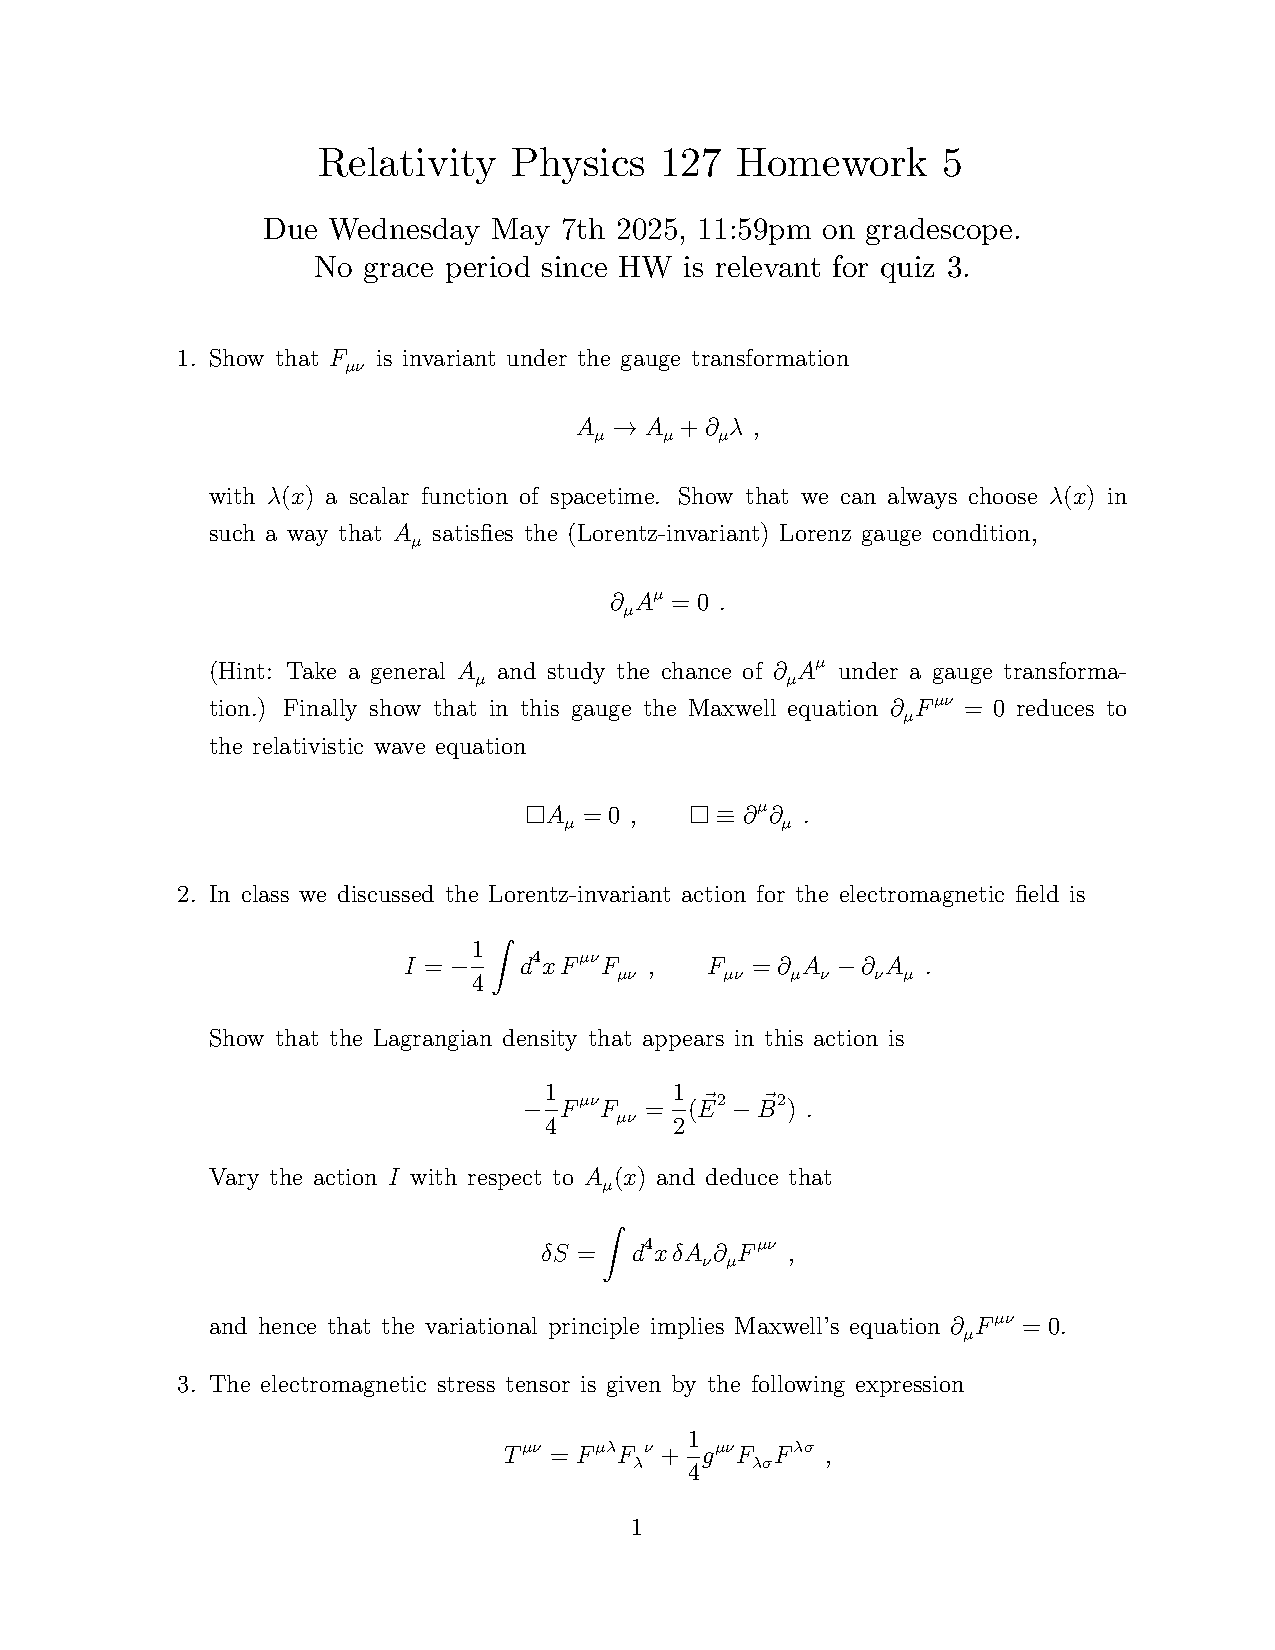
\includepdf[pages=-]{assignment.pdf}

\end{document}
